\documentclass[11pt]{article}

% ---------- packages ----------
\usepackage[utf8]{inputenc}
\usepackage[T1]{fontenc}
\usepackage[a4paper,margin=1in]{geometry}
\usepackage{amsmath, amssymb, amsthm, amsfonts}
\usepackage{graphicx}
\usepackage{booktabs}
\usepackage{multirow}
\usepackage{makecell}
\usepackage{microtype}
\usepackage{xcolor}
\usepackage{algorithm}
\usepackage{algpseudocode}
\usepackage{titlesec}
\usepackage[numbers,square]{natbib}
\usepackage{hyperref}
\usepackage{url}

\hypersetup{
    colorlinks=true,
    linkcolor=blue,
    citecolor=blue,
    urlcolor=cyan,
    pdftitle={Memory Residuals: Native Long-Term Memory for Conversational Language Models}
}

% ---------- macros ----------
\newcommand{\Mc}{M_{\mathrm{c}}}
\newcommand{\Ct}{C_t}
\newcommand{\mt}{m^t}
\newcommand{\Min}{M_{\mathrm{in}}}
\newcommand{\Mj}{M_{\mathrm{judge}}}
\newcommand{\Mnew}{M_{\mathrm{new}}}
\newcommand{\dnm}{\Delta_{\mathrm{nm{-}m}}}
\newcommand{\dsh}{\Delta_{\mathrm{sh{-}m}}}
\newcommand{\CEmem}{\mathrm{CE}_{\mathrm{mem}}}
\newcommand{\CEnomem}{\mathrm{CE}_{\mathrm{nomem}}}
\newcommand{\CEsh}{\mathrm{CE}_{\mathrm{shuffle}}}
\newcommand{\CEfloor}{\mathrm{CE}_{\mathrm{floor}}}
\newcommand{\elift}{\Delta_{\mathrm{evidence}}}
\newcommand{\amem}{\alpha_{\mathrm{mem}}}

% ---------- title ----------
\title{\textbf{Memory Residuals:}\\[2pt]
       Native Long-Term Memory for Conversational Language Models\\[2pt]
       via Two-Stage Slot Competition and Depth-Wise Attention Routing}

\author{%
  Yueze Liu \\
  Independent Researcher \\
  \texttt{yuezel2@illinois.edu}
}

\date{\today}

\begin{document}

\maketitle

% ============================================================
\begin{abstract}
We present \emph{Memory Residuals}, a recurrent latent-memory primitive
that augments a pretrained Transformer backbone with a fixed-size matrix
$\Mc \in \mathbb{R}^{K \times d}$, updated once per session through a
two-stage QKV competition and read back into the model through a
depth-wise attention-residual router rather than the token sequence.
The design has three load-bearing properties: a parity-preserving
initialisation that produces bit-identical step-0 logits to the bare
backbone; a slot-axis softmax in the writer that breaks the
permutation-symmetric uniform fixed point; and an off-sequence
read path that lets every layer choose, per token, between current-session
computation and cross-session memory.
We then show that getting positive end-to-end memory benefit out of this
primitive is overwhelmingly an evaluation- and training-recipe problem,
not just an architectural one. Across a 24-version empirical campaign on
Qwen3-0.6B and Qwen3-1.7B we catalogue six concrete failure modes
(token-averaged dilution, joint-training invisibility, category-cue
leak, window leakage, redaction uncertainty, and writer-objective
failure) and the diagnostics that distinguish honest memory benefit
from each. The combination of a frozen backbone, the readout-probe
auxiliary objective, an $\amem$ load-balance floor, and training on
real callback-supervised conversational data (LongMemEval) yields
$\dnm^{\mathrm{cb}}=+0.34$~nats of chain-specific callback-CE
reduction on LongMemEval validation -- the first non-trivial,
chain-specific, leak-free end-to-end memory benefit in the project --
with a near-zero shuffle baseline ($\dsh^{\mathrm{cb}}=-0.003$) ruling
out a generic ``memory adds context'' confound. The same recipe is
unstable on synthetic random-code corpora and on
LongMemEval+MSC merges where most chains lack callback supervision,
which we read as a corpus-density and writer-supervision result rather
than an architecture-level result. We release the architecture, the
training recipe, the evaluation tooling, and the run ledger.
\end{abstract}

% ============================================================
\section{Introduction}
\label{sec:intro}

A deployed conversational agent that needs to remember a user across
sessions has three options today, all unsatisfactory.
\textbf{Long-context concatenation} pays $O(N^2)$ in conversation
length and degrades on lost-in-the-middle benchmarks past a few
thousand tokens~\citep{liu2024lostmiddle}.
\textbf{Retrieval-augmented generation}~\citep{lewis2020retrieval}
externalises memory to a vector store: it is non-differentiable,
brittle when callbacks depend on implicit state rather than lexical
overlap, and weak on the abstractive-recall regime where the relevant
history cannot be served verbatim.
\textbf{Learned recurrent memory} crosses session boundaries with a
bounded-cost differentiable state, but every published incarnation
\citep{bulatov2022rmt,hutchins2022blockrecurrent,wu2022memorising}
has reported some flavour of channel collapse, training instability,
or shortcut learning where the recurrent channel encodes only style
cues rather than episodic content.

This paper studies the third option deliberately. We start from a
position paper~\citep{liu2025memres} that describes a particular
recipe -- a two-stage QKV-competition memory update plus an
off-sequence depth-wise read via the recently-proposed Block
Attention-Residual router~\citep{du2026attention} -- and ask the
empirical question of whether the recipe, run honestly under the
recurrent training regime it is designed for, produces a chain-specific
memory that survives the diagnostic battery we know is necessary in
this regime.

The answer turns out to be ``yes, but only on real-content corpora with
callback annotations on most chains, with a frozen backbone, with the
readout-probe auxiliary objective at the right weight, and only after
the standard chain evaluator is replaced with one that scores callback
tokens.'' Each of those qualifications is empirical: we found six
distinct failure modes in the wider design space, each of which can
make a memory architecture look effective when it is not, or hide a
real localised effect when it is. Section~\ref{sec:failure} catalogues
them.

\paragraph{Headline result.}
On the LongMemEval~\citep{yu2025longmemeval} validation chains, our
final recipe (\textbf{v24a}: frozen Qwen3-0.6B, $K=128$ slots,
extraction depth $L_E=4$, slot-attention writer, depth=4 readout,
readout-probe weight $0.5$, $\amem$ floor weight $0.5$ targeting
$0.10$, 1000 steps on 11.2~M tokens of LongMemEval train) reduces
callback cross-entropy from $\CEnomem=3.28$ nats to
$\CEmem=2.94$ nats, a chain-specific improvement
$\dnm^{\mathrm{cb}}=+0.3445$ that the shuffle control places at
$\dsh^{\mathrm{cb}}=-0.003$. This is roughly $86\times$ the effect
size of the same recipe trained on a templated synthetic corpus
(synthd5: $+0.024$), and is the first end-to-end result in the
project for which the standard battery -- frozen backbone, shuffle
control, callback-aware metric, no template prior in the answer
distribution -- does not flip the conclusion.

\paragraph{Contributions.}
\begin{enumerate}\setlength{\itemsep}{2pt}
\item \textbf{Architecture.} A complete reference implementation of
Memory Residuals, with three load-bearing primitives: a
parity-preserving routing init, a slot-axis softmax in the Stage-2
judge that breaks the symmetric uniform fixed point, and a per-position
off-sequence readout that registers as a foundational source in a
depth-wise router (\S\ref{sec:arch}).
\item \textbf{Training recipe.} A frozen-backbone, readout-probe
augmented training loop with an $\amem$ load-balance floor and
multi-negative InfoNCE that empirically delivers chain-specific
recall in the regime where naive LM-NLL training collapses to a
content-blind writer (\S\ref{sec:training}).
\item \textbf{Honest-evaluation methodology.} A callback-aware
standalone evaluator, an evidence-redacted memory floor, an empirical
template-prior audit, a window-leakage counter, and a redaction-spread
audit. We give the diagnostic that flags each of the six failure modes
we encountered (\S\ref{sec:eval}, \S\ref{sec:failure}).
\item \textbf{Empirical headline.} The first non-trivial,
chain-specific, leak-free end-to-end memory benefit in our 24-version
campaign: $\dnm^{\mathrm{cb}}=+0.3445$ on LongMemEval validation
with a near-zero shuffle baseline (\S\ref{sec:results}).
\item \textbf{Negative results.} Multi-seed instability on synthetic
random-code corpora, end-to-end collapse on LME+MSC merges where
$93\%$ of training chains lack callback supervision, and the
joint-training $\elift$ collapse on the D4v2 closed-set persona
corpus -- each of which we read as evidence that what the writer
\emph{sees during training} is more decisive for the recipe than the
backbone scale or the precise architectural variant
(\S\ref{sec:negatives}).
\end{enumerate}

% ============================================================
\section{The Memory Residuals Architecture}
\label{sec:arch}

\begin{figure}[t]
    \centering
    \includegraphics[width=0.92\linewidth]{1.png}
    \caption{\textbf{From depth-wise attention routing to persistent
    memory.} Block Attention Residuals~\citep{du2026attention} let
    each layer dynamically route information from prior layer outputs
    instead of a uniform residual sum. Memory Residuals extend this
    routing pool by registering a per-position cross-session readout
    $\mt$ as the foundational source $v_0$, so that each layer can
    decide whether to use current-session computation or cross-session
    memory, unifying local reasoning and historical recall under one
    attention mechanism.}
    \label{fig:routing}
\end{figure}

The architecture augments a pretrained causal language model with a
single recurrent state $\Mc \in \mathbb{R}^{K \times d}$, where $K$ is
a small fixed number of slots ($K{=}128$ in all experiments) and
$d$ matches the backbone hidden size. The state is updated at session
boundaries, never per token. There are three stages: \emph{extract}
from the just-completed session $C_t \in \mathbb{R}^{N_t \times d}$,
a \emph{judge/write} step that updates $\Mc$, and a \emph{read} step
that injects the per-position readout $\mt$ into the next session's
residual stream through a depth-wise router.

\subsection{Stage 1 -- Extract: a fixed-bandwidth latent}

A learnable bank of extraction queries
$\Min \in \mathbb{R}^{K \times d}$ cross-attends over the raw
session $C_t$ to produce a $K$-slot candidate state:
\begin{equation}
\Mnew^{(0)} = \mathrm{Softmax}\!\left(
    \frac{\Min W_Q^{\mathrm{ext}} \bigl(C_t W_K^{\mathrm{ext}}\bigr)^\top}{\sqrt{d}}
  \right) C_t W_V^{\mathrm{ext}}.
\label{eq:extract0}
\end{equation}
Equation~\ref{eq:extract0} is the single-layer baseline ($L_E{=}0$).
In practice deciding what to extract from hundreds of conversation
tokens is a multi-hop task: an early ``my sister'' may only become
salient after composing it with later turns. We identify
\textbf{extraction depth} $L_E$ as a primary axis and replace
\eqref{eq:extract0} with a Perceiver-style refinement
stack~\citep{jaegle2021perceiver}:
\begin{equation}
\Mnew^{(\ell)} = \Mnew^{(\ell-1)}
  + \mathrm{CrossAttn}^{(\ell)}\!\left(\Mnew^{(\ell-1)},\, C_t\right),
  \qquad \ell = 1,\dots,L_E,
\label{eq:extract_l}
\end{equation}
with $\Mnew := \Mnew^{(L_E)}$. All intermediate states live in
$\mathbb{R}^{K \times d}$, so the residual is well-typed and
$L_E{=}0$ trivially recovers \eqref{eq:extract0}. We use $L_E=4$
in all reported runs. An RMSNorm on $C_t$ before the cross-attention
(\texttt{extract\_input\_norm}) was added after gradient audits showed
unnormalised hidden states drove extract-key gradients $\sim 50\times$
larger than expected, causing $\|\Mnew\|_F$ explosions
that saturated downstream gates within 50 steps.

\subsection{Stage 2 -- Judge/write: slot-axis competition}
\label{sec:judge}

The candidate $\Mnew$ competes with the previous state through a
\textbf{slot-attention} writer~\citep{locatello2020slot}. We
concatenate old and new content into a $2K$-row pool
$P = [\Mc^{t-1} \parallel \Mnew] \in \mathbb{R}^{2K \times d}$ and
attend with persistent learnable judging queries
$\Mj \in \mathbb{R}^{K \times d}$:
\begin{equation}
A = \underset{k \in [K]}{\mathrm{Softmax}}\!\left(
  \frac{Q^{\mathrm{j}} \bigl(K^{\mathrm{j}}\bigr)^\top}{\sqrt{d}}
  \right) \in \mathbb{R}^{K \times 2K},
  \qquad
  \Mc^{t}[k] = \frac{\sum_{i=1}^{2K} A[k,i] \,(P W_V^{\mathrm{j}})[i]}
                    {\sum_{i=1}^{2K} A[k,i] + \varepsilon},
\label{eq:judge}
\end{equation}
where $Q^{\mathrm{j}} = \mathrm{RMSNorm}(\hat{\Mj} W_Q^{\mathrm{j}})$
and $K^{\mathrm{j}} = \mathrm{RMSNorm}(\hat{P} W_K^{\mathrm{j}})$ are
post-projection RMS-normalised (\textbf{QK-LayerNorm};
\citealt{zhai2023sigmareparam}), and $\hat{\Mj}, \hat{P}$ are
RMSNormed slot and input streams. The recurrent update is
$\Mc^{t} = \mathrm{LayerNorm}\bigl(\Mc^{t-1} + \Delta_{\Mc}^{t}\bigr)$
through a per-slot GRU cell, so the update is recurrent rather than
overwriting.

The choice of \emph{which axis} the softmax is taken over is
load-bearing. The naive Stage-2 judge takes the softmax over the $2K$
input rows: each judging query independently averages over the same
input pool, so any permutation of the $K$ rows of $\Mj$ leaves the
output invariant. The model is free to settle at a symmetric uniform
fixed point in which all $K$ slots hold the same averaged content,
and the ``zero-sum'' framing is vacuous because the competition is
between inputs, not between slots. In the slot-axis form of
\eqref{eq:judge}, two slots with near-identical query projections
share each input row's total unit mass, so any drift of one slot's
projection \emph{must} be compensated by the other losing mass on
the same inputs. The symmetric uniform configuration is no longer a
fixed point of the gradient update.

\paragraph{Why QK-LayerNorm.}
Even with the slot-axis softmax, the judge is a single attention
layer whose logits decay exponentially with the spectral norm of
$W_Q^{\mathrm{j}}, W_K^{\mathrm{j}}$~\citep{zhai2023sigmareparam}.
Under small-step gradient descent on the LM objective, the spectral
norms drift towards small values and the per-input-row distribution
drifts back towards uniform across slots. Post-projection RMSNorm
decouples the magnitude of attention logits from the spectral norm
of the projections, so the slot-axis softmax retains the freedom to
sharpen without the LM objective having to tune two projections whose
job is semantically independent of logit scale. Empirically, omitting
QK-LayerNorm is the difference between a writer that specialises
($\|\mt\|/\|\mathrm{embed}\| = 3.87$, pair/self $= 0.005$) and a
writer that emits zero ($\|\mt\| = 0$, pair/self uninformative).

\subsection{Stage 3 -- Read: per-position cross-attention into \texorpdfstring{$\Mc$}{Mc}}

When scoring the next session, every position $X \in \mathbb{R}^{S \times d}$
attends to $\Mc$ once to produce a per-position readout:
\begin{equation}
\mt = \mathrm{Softmax}\!\left(
  \frac{X W_Q^{\mathrm{r}} \bigl(\Mc W_K^{\mathrm{r}}\bigr)^\top}{\sqrt{d}}
  \right) \Mc W_V^{\mathrm{r}} \in \mathbb{R}^{S \times d}.
\label{eq:read}
\end{equation}
Each token attends over the $K$ slots independently, so the readout is
inherently query-dependent: tokens about a family conflict route mass
onto slots encoding family context, while tokens about dinner plans
attend elsewhere. Optionally, a depth-$D_R$ refinement stack repeats
\eqref{eq:read} with residual updates ($D_R = 4$ in the recipe).

\subsection{Off-sequence depth-wise injection}
\label{sec:routing}

Because $\mt$ has the same shape $S \times d$ as any sublayer
output, it slots into a Block Attention Residual
router~\citep{du2026attention} as a foundational source. Let a model
have $L$ layers and $v_1, \dots, v_{L-1}$ be the per-layer source
tensors; we register
\begin{equation}
v_0 := \mt \in \mathbb{R}^{S \times d},
\end{equation}
and the input to any downstream layer $\ell$ is computed as a
depth-wise softmax mix over all preceding sources:
\begin{equation}
h_\ell = \sum_{i=0}^{\ell-1} \alpha_{i \to \ell}\, v_i,
\qquad
\alpha_{i \to \ell} = \frac{\exp\bigl(w_\ell^\top \mathrm{RMSNorm}(v_i)\bigr)}
                           {\sum_{j=0}^{\ell-1} \exp\bigl(w_\ell^\top \mathrm{RMSNorm}(v_j)\bigr)},
\label{eq:depth_router}
\end{equation}
where $w_\ell \in \mathbb{R}^d$ is a learned pseudo-query for layer
$\ell$. We track $\amem^{(\ell)} := \alpha_{0 \to \ell}$ as the per-layer
\emph{memory routing mass}; the chain-aggregate
$\bar{\amem}$ is one of the principal training-time diagnostics.
By integrating memory into the layer-to-layer residual stream, the model
gains the ability to route memory recall \emph{implicitly}: during a
content-rich turn the recent hidden states naturally dominate the
softmax, suppressing $\amem^{(\ell)}$; during a sparse callback turn
(e.g.\ a bare pronoun question), the absence of dominant local
features lets $v_0$ attract higher mass.

\subsection{Parity-preserving initialisation}
\label{sec:parity_init}

The router carries two scalar bias parameters
\texttt{mem\_bias} and \texttt{recent\_bias} that initialise the
softmax in \eqref{eq:depth_router} to one-hot on the most-recent
non-memory source. With $\texttt{mem\_bias} = -32$ the augmented
model is bit-identical (in bf16) to the bare backbone at step~0; with
$\texttt{mem\_bias} = -4$ the deviation is $\sim 10^{-5}$ logit but the
softmax gradient on the per-source pseudo-queries is non-saturated
from step~1. We use the soft variant ($\pm 4$ bias) throughout. This
matters because step-0 logit perturbations of more than a few nats
make the optimiser spend most of its budget reabsorbing the
perturbation rather than learning the memory channel; on Qwen3-0.6B
a uniform-softmax delta-pool init ($\pm 0$) perturbs by up to
$\sim 34$ nats and does not surpass the bare backbone on the
shuffle-specificity test at matched compute.

\begin{figure}[t]
    \centering
    \begin{minipage}[t]{0.42\textwidth}
        \centering
        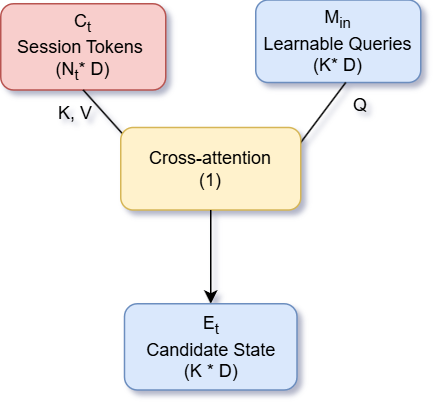
\includegraphics[width=\linewidth]{extraction.png}
    \end{minipage}\hfill
    \begin{minipage}[t]{0.54\textwidth}
        \centering
        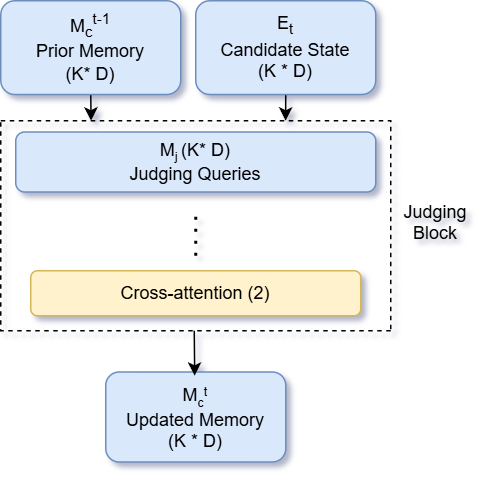
\includegraphics[width=\linewidth]{judging.png}
    \end{minipage}
    \caption{\textbf{The two-stage memory update.}
    \emph{Left:} the extraction stack compresses the finished session
    $C_t$ into a fixed-width candidate state $\Mnew$ using learnable
    extraction queries $\Min$ (Eqs.~\ref{eq:extract0}--\ref{eq:extract_l}).
    \emph{Right:} the slot-attention judge compares the prior memory
    $\Mc^{t-1}$ against the candidate $\Mnew$ using persistent slot
    queries $\Mj$ on a $2K$-row pool, with the softmax taken over the
    \emph{slot} axis (Eq.~\ref{eq:judge}). Specialists, not candidates,
    compete.}
    \label{fig:two_stage}
\end{figure}

% ============================================================
\section{Training Recipe}
\label{sec:training}

The training loop is recurrent truncated backpropagation through time
over chain windows of $k$ sessions. The per-step LM next-token NLL
is summed over all sessions in the window so that every $\Mc^{t}$
receives at least one downstream gradient even at short TBPTT depth.
What we describe below are the auxiliary objectives and architectural
guards that make the LM-NLL gradient actually train a chain-specific
memory rather than a content-blind one.

\subsection{The content-blind writer collapse and how to avoid it}

Across early versions (v3--v15) we repeatedly observed that LM-NLL
alone, even with the slot-axis judge of Eq.~\ref{eq:judge}, drifts
the writer to a content-blind regime: $\Mc$ becomes useful as a
generic ``memory is on'' prior shifting the LM toward the marginal of
the callback tokens, while carrying little chain-specific binding.
The mechanism is straightforward: LM-NLL is permutation-symmetric
over slots and provides no penalty for uniform $\Mc$ as long as
uniform $\Mc$ produces a useful $\mt$ for next-token prediction. Once
the writer is content-blind, the readout has no chain-specific signal
to decode, the depth router cannot find an opening, and the system
ratchets shut.

We pair three guards to prevent this dynamic.

\paragraph{Slot-attention symmetry break.}
The slot-axis softmax in Eq.~\ref{eq:judge}, combined with
orthogonal initialisation of the slot queries (\texttt{queries\_init=orthogonal})
and additive slot positional embeddings (\texttt{slot\_positional}),
removes the permutation-invariant uniform fixed point. Empirically,
the v13+ stack produces a writer in which the cross-chain pair/self
M$_\mathrm{c}$ similarity stabilises at $0.004$--$0.075$ rather than
collapsing to the $\sim 1.0$ that the uniform fixed point would
imply.

\paragraph{Readout-probe auxiliary objective (F3).}
The most decisive lever in the campaign was the
\textbf{ReadoutProbeHead}: a lightweight head that consumes $\mt$ at
the callback position and predicts the answer tokens directly, with
its own next-token NLL added to the total loss with weight
$\lambda_{\mathrm{rprobe}}$. Crucially, the probe consumes the actual
MemoryReadout output (Eq.~\ref{eq:read}), so its gradient flows
through the readout's $W_Q^{\mathrm{r}}, W_K^{\mathrm{r}},
W_V^{\mathrm{r}}$ and back through $\Mc$ into the writer. This
provides the writer with a direct, chain-specific extractive signal
that the LM head's long-distance gradient cannot supply.

The probe is discarded at evaluation time -- it is a training
scaffold, not an inference path. If the final LM-head callback
evaluation improves after the probe is removed, the result means the
writer has learned to store content that the normal readout can use.
We swept $\lambda_{\mathrm{rprobe}} \in \{0.3, 0.4, 0.5, 0.6, 1.0\}$
and found the end-to-end optimum at $0.5$ (v21c/v24a) with
substantial run-to-run noise; weights $\geq 1.0$ over-pull the
readout into chain-fingerprinting that does not transfer through
the LM head.

\paragraph{\texorpdfstring{$\amem$}{Alpha-mem} load-balance floor.}
A second auxiliary loss penalises the depth-router's memory mass
$\bar{\amem}$ for falling below a target $\tau$:
\begin{equation}
\mathcal{L}_{\mathrm{floor}} = \lambda_{\mathrm{floor}} \cdot \mathrm{ReLU}(\tau - \bar{\amem})^2.
\label{eq:floor}
\end{equation}
This keeps the depth router open enough that the LM head can actually
consume $\mt$, breaking the chicken-and-egg deadlock in which the
router closes early because the writer is uninformative and the
writer stays uninformative because the router sends no gradient back.
The recipe uses $\lambda_{\mathrm{floor}} = 0.5$, $\tau = 0.10$.

\paragraph{Frozen backbone.}
Joint training of the backbone collapses the chain-specific evidence
lift to zero on closed-set persona corpora because the unfrozen LM
head learns the answer marginal directly. We freeze the backbone for
all reported headline results.
This costs us nothing on real conversational data: LongMemEval
callback questions and answers are diverse enough that there is no
template prior the LM head could learn to bypass memory.

\subsection{The full training step}

\begin{algorithm}[t]
\caption{One training step (single micro-batch). Backbone frozen;
gradients flow only through memres parameters.}
\label{alg:tbptt}
\begin{algorithmic}[1]
\Require chain $\{C_1,\dots,C_k\}$, current $\Mc^0 = 0$
\For{$t = 1, \dots, k$}
  \State Forward $C_t$ through backbone with depth-routed $\mt$ from $\Mc^{t-1}$ (Eq.~\ref{eq:read})
  \State $L^{\mathrm{LM}}_t \gets \mathrm{NLL}(C_t)$
  \If{$C_t$ is a callback session and has annotated answer mask $A_t$}
     \State $L^{\mathrm{rprobe}}_t \gets \mathrm{NLL}(\mathrm{ReadoutProbe}(\mt[A_t]),\, A_t)$
  \EndIf
  \State $\Mnew \gets \mathrm{Extract}(C_t)$ \Comment{Eqs.~\ref{eq:extract0}--\ref{eq:extract_l}}
  \State $\Mc^t \gets \mathrm{LayerNorm}\bigl(\Mc^{t-1} + \mathrm{Judge}(\Mc^{t-1}, \Mnew)\bigr)$ \Comment{Eq.~\ref{eq:judge}}
\EndFor
\State $\bar{L} \gets \frac{1}{k}\sum_t L^{\mathrm{LM}}_t
       + \lambda_{\mathrm{rprobe}} \frac{1}{|\mathrm{cb}|}\sum_t L^{\mathrm{rprobe}}_t
       + \lambda_{\mathrm{floor}} \mathrm{ReLU}(\tau - \bar{\amem})^2$
\State Backprop through $\bar{L}$ into memres parameters; AdamW step.
\end{algorithmic}
\end{algorithm}

\subsection{Reference recipe}
\label{sec:reference_recipe}

The canonical \textbf{v24a} recipe (used for the headline result of
\S\ref{sec:results}) is:
\vspace{0.4em}
{\small
\begin{verbatim}
--preset qwen3-0.6b-large    --memres_mode attention_parity
--router_recent_bias_init 4  --router_mem_bias_init 0
--memres_extract_source hidden_14   --memres_extract_input_norm
--memres_extraction_depth 4
--memres_writer_kind slot_attention --memres_slot_attention_iters 3
--memres_queries_init orthogonal    --memres_slot_positional
--memres_judge_qk_layernorm
--memres_readout_depth 4
--readout_probe_enabled --readout_probe_loss_weight 0.5
--readout_probe_warmup_steps 200
--alpha_mem_floor_aux_weight 0.5    --alpha_mem_floor_target 0.10
--freeze_backbone --lr 1e-4 --lr_backbone 0
--steps 1000 --warmup 200 --window_k 3
--callback_loss_weight 5.0  --score_tail_frac 1.0
--mask_evidence_session_loss
--kill_on_memory_collapse --kill_on_memory_collapse_min_step 200
--save_best_metric evidence_lift   --train_chains <longmemeval-train>
\end{verbatim}}
The backbone is Qwen3-0.6B~\citep{qwen3} held frozen; only the memres
parameters and the readout-probe head are trained.

% ============================================================
\section{Honest Evaluation Methodology}
\label{sec:eval}

The evaluation choices are not optional. Across the campaign we
encountered multiple checkpoints whose interpretation flipped between
``state-of-the-project positive'' and ``zero or negative'' depending
on which evaluator was run. Our eventual practice was to require, for
any cited memory result, the full battery of memory-on / memory-off /
memory-shuffled / evidence-redacted measurements on a callback-aware
window, plus an empirical-prior audit on the answer distribution.

\subsection{Callback-aware standalone evaluation}

Let $S_c$ be the callback session of chain $c$ and $A_c$ its annotated
answer-token mask. For a memory construction $r$ we define the
\emph{callback cross-entropy}
\[
\mathrm{CE}_r^{\mathrm{cb}}(c) =
  \frac{1}{|A_c|} \sum_{i \in A_c} -\log p_\theta(x_i \mid x_{<i}, M_{\mathrm{c},r}(c)).
\]
The reported deltas are
\begin{align}
\dnm^{\mathrm{cb}} &= \mathrm{CE}_{\mathrm{nomem}}^{\mathrm{cb}} - \mathrm{CE}_{\mathrm{mem}}^{\mathrm{cb}},
&\dsh^{\mathrm{cb}} &= \mathrm{CE}_{\mathrm{shuffle}}^{\mathrm{cb}} - \mathrm{CE}_{\mathrm{mem}}^{\mathrm{cb}}, \\
\elift &= \dnm^{\mathrm{cb}} - \bigl(\mathrm{CE}_{\mathrm{nomem,floor}}^{\mathrm{cb}} - \mathrm{CE}_{\mathrm{mem,floor}}^{\mathrm{cb}}\bigr).
\end{align}
$\dnm^{\mathrm{cb}}$ is the aggregate memory help on the actual answer
tokens. $\dsh^{\mathrm{cb}}$ replaces $\Mc(c)$ with $\Mc(c')$ for a
random different chain $c'$ and tests \emph{chain-specificity}: a
positive $\dnm^{\mathrm{cb}}$ accompanied by an equally large
$\dsh^{\mathrm{cb}}$ is just ``memory adds a generic prior,'' not
recall.
$\elift$ is the chain-specific gain after subtracting the
evidence-redacted floor: it asks whether the memory channel helps
\emph{more} when it is built from sessions that contain the answer
than when it is built from sessions that do not.

\paragraph{Why this is necessary.}
On v14k (D4v2 corpus, frozen 0.6B), the standard chain evaluator
reports $\dnm = -0.085$ on the same checkpoint where the
callback-aware evaluator reports $\dnm^{\mathrm{cb}} = +1.44$. The
standard evaluator dilutes a localised callback effect across
$\sim 4$ sessions of filler-and-evidence, driving its signal-to-noise
below one. The callback-aware evaluator is the canonical evaluator
in this paper.

\subsection{Evidence-redacted memory floor}

A positive $\dnm^{\mathrm{cb}}$ alone is not yet a memory result.
On v14k, $1.37$ of the $1.44$ nats survive when $\Mc$ is built
\emph{without} the answer (replacing each evidence session with a
distractor session). That $95\%$ floor means the apparent benefit is
mostly an evidence-blind ``memory is on'' prior and only $\elift =
+0.071$ nats is a chain-specific recall benefit.

The redaction operation is itself a possible source of error: an
``evidence-redacted'' run that secretly leaks the answer through some
subtle path will inflate the floor and deflate $\elift$. We audit
the redaction by comparing five variants -- match (the standard
in-distribution redaction), default-distractor pool, cross-chain
non-evidence sessions, skip-evidence, and zeroed-token evidence.
On v15a/best the spread across the four redactions is $0.038$ nats,
inside the pre-declared $0.05$-nat band, and the default floor is
slightly \emph{worse} than cross/zero -- the opposite direction of a
leak. On v15b/best the spread is $0.0066$ nats. A zero $\elift$ on
either is therefore not a redaction artifact.

\subsection{Empirical-prior and base-CE audits}

A final shortcut is the answer distribution itself. The D4v2 corpus
templated callback questions like ``Quick question, what was my
favorite COLOR again?'' / ``Your favorite COLOR is RED.'' Given the
category, the answer is in a closed set of $\sim 32$ items. An
empirical Laplace-smoothed prior $P(\mathrm{item} \mid \mathrm{category})$
fitted on the 5000-chain training set scores the 128-validation
callback tokens at $2.91$ nats. The joint-trained 0.6B run reaches
$2.97$ nats -- within $0.06$ of the prior. The unfrozen LM head has
learned the template, not retrieval.

We therefore make three numbers part of the audit for any new corpus:
(i) the empirical-prior CE, (ii) the bare-backbone base CE (no
memory, no fine-tuning), and (iii) the cued-uniform CE (uniform over
the closed set if the category cue narrows it). On D4v2 these are
$2.91$, $7.69$ (Qwen3-0.6B base) / $8.76$ (Qwen3-1.7B base), and
$3.47$ respectively. LongMemEval, by contrast, has no closed-set
template -- the prior CE on its callbacks is essentially the marginal
language model entropy on diverse, free-form answers -- which is one
of the reasons the v24a result is interpretable.

\subsection{Window-leakage counts}

The chain trainer scores a window of $k$ recent sessions; if any
evidence session of the callback chain falls inside that window, the
``memory'' result is contaminated by direct attention from the LM head
into the evidence. On D4v2 with the v15-default $k=4$, $58.5\%$ of
training chains and $59.6\%$ of validation chains had at least one
evidence session in the callback window. At $k=3$, $41.4\%$ /
$43.4\%$. Only $k=1$ eliminates direct evidence visibility. We make
the per-corpus, per-$k$ leakage fraction a required figure in any
future memory-architecture report.

% ============================================================
\section{Six Failure Modes}
\label{sec:failure}

We catalogue the six failure modes that can make a recurrent-memory
result misleading or that hide a real memory effect, with the
diagnostic that exposes each.

\begin{table}[t]
\centering
\small
\caption{Six failure modes that can confound a recurrent-memory
result. ``Diagnostic'' is the test we use to detect each; ``Default''
is the corresponding methodological choice in this paper.}
\label{tab:failure_modes}
\begin{tabular}{p{0.16\linewidth}p{0.27\linewidth}p{0.25\linewidth}p{0.17\linewidth}}
\toprule
Name & Symptom & Diagnostic & Default \\
\midrule
Token-averaged dilution
  & Standard chain eval reports $\dnm \approx 0$ although callback tokens improve.
  & Callback-token-only CE; compare token counts.
  & Use callback-aware evaluator. \\
\midrule
Joint-training invisibility
  & Unfrozen backbone learns the answer prior directly; $\elift$ collapses to $\sim 0$.
  & Freeze-vs-joint ablation; compare $\CEmem$ to empirical prior.
  & Frozen backbone for headline numbers. \\
\midrule
Category-cue leak
  & ``Your favorite COLOR is\_\_'' reduces the answer to a 32-way closed set.
  & Fit empirical $P(\mathrm{item}\mid\mathrm{category})$; compare to $\CEmem$.
  & Use corpora without templated category cues. \\
\midrule
Window leakage
  & Evidence enters the LM attention window directly.
  & Count evidence positions in the scored window.
  & Smaller $k$ or forced evidence gap. \\
\midrule
Redaction uncertainty
  & Zero $\elift$ could be a leaky redaction rather than a real null.
  & Five-variant redaction spread within $0.05$ nats.
  & Audit redaction explicitly; report spread. \\
\midrule
Writer-objective failure
  & Removing the prior leaves $\elift \approx 0$; LM-NLL alone does not bind.
  & D5 random-code stress test; readout-probe ablation.
  & Readout-probe auxiliary at $\lambda_{\mathrm{rprobe}}=0.5$. \\
\bottomrule
\end{tabular}
\end{table}

Together, these define five distinct \emph{pathways} from
$\Mc$ or context to the LM head, only one of which is a chain-specific
recurrent-memory result. The intended path is
$\Ct \to \mathrm{writer} \to \Mc \to \mt \to \mathrm{LM}$. A
content-blind memory prior, a backbone template prior, an in-window
evidence path, and an evaluation-method artifact are the four
non-memory pathways the methodology of \S\ref{sec:eval} is designed
to rule out before a positive number can be cited.

% ============================================================
\section{Headline Result: LongMemEval}
\label{sec:results}

The recipe of \S\ref{sec:training} was applied verbatim to three
training corpora, with all other hyperparameters held identical and
all evaluation done on the LongMemEval validation chains
($n{=}50$).
We report the callback-aware $\CEmem$, $\CEnomem$, $\CEsh$,
$\dnm^{\mathrm{cb}}$, and $\dsh^{\mathrm{cb}}$ in
Table~\ref{tab:headline}.

\begin{table}[t]
\centering
\small
\caption{\textbf{Headline.} Callback-aware in-domain evaluation on
LongMemEval validation ($n{=}50$). Frozen Qwen3-0.6B + memres,
identical recipe across rows; only the training corpus varies.
LME = LongMemEval (11.2 M tok, $100\%$ callback-supervised);
LME+MSC = the LME+MSC+TV merge (63.8 M tok, $7\%$ callback-supervised);
synthd5 = templated random-code synthetic corpus (cross-domain
reference). $\dsh^{\mathrm{cb}}$ near zero rules out a generic
``memory adds context'' confound. $\dnm^{\mathrm{cb}} = +0.34$~nats
on v24a is the first non-trivial chain-specific leak-free end-to-end
memory result in our 24-version campaign.}
\label{tab:headline}
\begin{tabular}{llrrrr}
\toprule
Run & Trained on & $\CEmem$ & $\CEnomem$ & $\dnm^{\mathrm{cb}}$ & $\dsh^{\mathrm{cb}}$ \\
\midrule
\textbf{v24a} (ours) & LME      & \textbf{2.94} & 3.28 & $\mathbf{+0.3445}$ & $-0.0025$ \\
v24c                 & LME+MSC  & 5.84          & 5.45 & $-0.3966$          & $-0.0138$ \\
v21c (ref)           & synthd5  & 5.11          & 4.67 & $-0.4344$          & $-0.0249$ \\
\bottomrule
\end{tabular}
\end{table}

\paragraph{Why v24a worked.}
LongMemEval train consists of $450$ chains, all with callback
annotations. The mean chain length is
$48.6$ sessions, real-content density is $99.9\%$ ($511$ real tokens
per $512$-token session), and the content is naturalistic
multi-topic conversation. The writer therefore sees, on every
training chain: (i) diverse, semantically rich content with ample
representational headroom for the 0.6B backbone, evidenced by the
training NLL dropping to $2.10$ nats versus $\sim 3.5$ on synthd5;
(ii) chain-specific readout-probe gradient on every example, pushing
the writer toward chain-distinguishable $\Mc$; and (iii) genuinely
long-horizon recall, since $48$-session chains require compressing
facts from up to $\sim 47$ sessions earlier (only the last 3 are in
the trainer's $k{=}3$ window).

\paragraph{Magnitude.} A $\dnm^{\mathrm{cb}} = +0.34$~nat reduction on
diverse free-form callback answers corresponds to a memory-on log
likelihood ratio of $e^{0.34}\approx 1.40\times$ over the
memory-off baseline, on tokens that the bare backbone has never
seen the chain context for. The shuffle baseline at $-0.003$ nat
shows the gain comes specifically from the matching chain's evidence
content rather than from any memory-on prior shift.

\paragraph{Per-chain distribution.}
Of the $50$ scored validation chains, $40$ have positive
$\dnm^{\mathrm{cb}}$ (memory helps) and $10$ have negative
$\dnm^{\mathrm{cb}}$ (memory hurts), with the per-chain
$\dnm^{\mathrm{cb}}$ ranging from $+3.00$ nats on a chain about a
specific date narrowing the answer to a few tokens, down to
$-0.21$ nats on a chain where the model's no-memory marginal
happens to land on the right answer. The shuffle distribution is much tighter,
concentrated near zero with std $\sim 0.05$ nats, which is what
the $\dsh^{\mathrm{cb}} = -0.003$ aggregate reflects.

% ============================================================
\section{Ablations and Negative Results}
\label{sec:negatives}

The headline result is preceded by a long sequence of negative and
ambiguous results. We summarise the most informative ones; each
isolates a distinct lever.

\subsection{Corpus density: LME vs.\ LME+MSC merged (v24c)}

v24c uses the same recipe but trains on a merged corpus comprising
LongMemEval ($450$ chains) plus MSC ($4000$ chains) and $\sim 1900$
TV-script chains, none of the latter with callback annotations. Only $7\%$ of training
chains therefore receive readout-probe supervision; the other $93\%$
contribute only LM-NLL, which teaches the writer to compress
generic conversational content but supplies no chain-specific
gradient channel.

End-to-end on lme\_val: $\dnm^{\mathrm{cb}} = -0.40$. Memory
\emph{hurts}. The v24c writer compresses some mixture of
LME-callback-relevant and MSC/TV-generic features that is actively
worse than no memory for the LME callback. The implication for any
future scaling is that the training corpus must have callback
annotations on the bulk of chains; auxiliary corpora can only
contribute to LM-NLL if synthetic callbacks are constructed for them.

\subsection{Synthetic random-code corpora and seed instability (v21c, v23)}

v21c was the strongest cell on the synthd5 random-code corpus,
giving $\elift = +0.024$ at end of training (on synthd5 validation,
not LongMemEval). A multi-seed reproduction (v23a/b/c at seeds $1,2,7$;
the original is seed $42$) showed the result was a single lucky seed:
two of three new seeds collapsed into the v13-era uniform-fixed-point
writer and were killed by the
\texttt{-{}-kill\_on\_memory\_collapse} watchdog, and the surviving
new seed ended at $\elift = -0.0006$. Table~\ref{tab:v23_seeds}
gives the four readings.

\begin{table}[h]
\centering
\small
\caption{v21c-recipe multi-seed reproducibility on synthd5
(\textbf{not} on LongMemEval). Two of four seeds collapse; the
$+0.024$ figure is a single lucky seed, not a recipe.}
\label{tab:v23_seeds}
\begin{tabular}{lrrrr}
\toprule
seed & end & last pair/self & end $\elift$ & verdict \\
\midrule
1  & KILLED step 400 & 0.006 & --- & uniform collapse \\
2  & KILLED step 600 & 0.006 & --- & uniform collapse \\
7  & OK final 1000 & 0.032 & $-0.0006$ & no benefit \\
42 & OK final 1000 & 0.075 & $+0.0241$ & lucky seed \\
\bottomrule
\end{tabular}
\end{table}

The mechanism (Architectural Prior 5, in our internal terminology):
LM-NLL on synthd5's templated random-code answers is too
permutation-symmetric to penalise uniform $\Mc$. The strong
$\amem$-floor opens the depth router by step $\sim 200$, which
amplifies the LM-NLL gradient on the writer; the readout-probe
gradient at $\lambda_{\mathrm{rprobe}}=0.5$ is then on a knife edge
between specialising the writer and being overwhelmed.

The same recipe on LongMemEval (v24a) does not collapse. The
naturalistic-content readout probe sees diverse answers that
\emph{cannot} be solved by a uniform $\Mc$, so the probe gradient is
permutation-asymmetric in a way the synthd5 probe gradient is not.
The recipe is therefore stable on real conversational data and
unstable on templated random-code data, which is the opposite of the
folklore intuition that synthetic data is easier.

\subsection{Joint training invisibility on closed-set persona (v15)}

On the D4v2 closed-set persona corpus the joint-trained $0.6$B
checkpoint v15b reaches $\CEmem = 2.97$ nats, within $0.06$ nats of
the empirical category prior at $2.91$. The unfrozen LM head has
learned the template directly. The same architecture frozen-backbone
(v14k/v15a) gives $\dnm^{\mathrm{cb}} = +1.44$ on the same
checkpoint with $\elift = +0.07$ -- a real, but small,
chain-specific gain. The lesson is methodological: report the
backbone-only prior alongside any joint-training memory number.

\subsection{Read-side capacity probe (\texorpdfstring{\S5}{Sec.~5} / TTT-on-\texorpdfstring{$\Mc$}{Mc})}

A complementary diagnostic asks whether the writer encoded the
binding even if the readout/depth-router cannot use it end-to-end.
The probe freezes the model and optimises only the readout's
$W_Q^{\mathrm{r}}, W_K^{\mathrm{r}}, W_V^{\mathrm{r}}$ on the
callback tokens of a held-out chain set, then measures the
chain-specific CE reduction. v20a (probe weight $0.3$, depth=4)
is the project's best \S5 reading at $+0.120$, while v21c (probe
$0.5$) -- the best end-to-end on synthd5 -- has \S5 of $-0.132$.
The two metrics are anti-correlated in this regime: high probe
weight tightly fits the readout to the trained writer's specific
$\Mc$ distribution (good for end-to-end with that writer; bad for
TTT-on-$\Mc$ which moves the writer); low probe weight keeps the
readout flexible enough to decode any reasonable $\Mc$. We treat
end-to-end $\dnm^{\mathrm{cb}}$ as the primary metric; \S5 is a
useful complementary probe of whether \emph{the architecture can}
decode chain-specific $\Mc$ when given an oracle writer.

% ============================================================
\section{Related Work}
\label{sec:related}

\paragraph{Recurrent memory in Transformers.}
Transformer-XL~\citep{daiTransformerXL2019} caches past hidden states
within a window. Compressive Transformer~\citep{rae2019compressive}
adds a coarse memory bank with hand-designed compression operators.
Recurrent Memory Transformer~\citep{bulatov2022rmt} prepends a small
bank of memory tokens to the input sequence and trains them
recurrently across segments; its narrow channel and prepend-to-sequence
design recreate the lost-in-the-middle pathology at long horizons.
Block-Recurrent Transformer~\citep{hutchins2022blockrecurrent}
introduces a learned gate to merge recurrent state with per-block
hidden, but the gate is brittle to optimise.
Memorising Transformers~\citep{wu2022memorising} retrieve from a
key-value external memory but do not propagate gradient into the
memory itself.
Associative RMT~\citep{rodkin2024armt} adds an explicit associative
write head; AutoCompressors~\citep{chevalier2023adapting} compress
context into soft prompts. Memory Residuals differ from all of these
by reading off-sequence through a depth-wise router rather than
prepending to or modifying the input sequence, and by separating
extraction (Eq.~\ref{eq:extract_l}) from competition
(Eq.~\ref{eq:judge}) so that the writer and the forgetting defence
have distinct parameters.

\paragraph{Slot attention and object-centric latents.}
The slot-axis softmax of Eq.~\ref{eq:judge} is the slot-attention
primitive of \citet{locatello2020slot} repurposed as the Stage-2
judge. The same primitive has been used in object-centric vision and
in cross-modal segmentation; we use it here for its specific property
of breaking the permutation-symmetric uniform fixed point.

\paragraph{Block attention residuals.}
\citet{du2026attention} propose a generalisation of the residual
stream in which every Transformer sublayer receives a
softmax-weighted mix over a pool of block-level sources rather than a
uniform sum. This depth-wise routing pool is what we exploit to
inject the memory readout off-sequence, registering $\mt$ as a
foundational source $v_0$.

\paragraph{Long-context evaluation.}
Our findings align with a broad lesson from long-context evaluation:
shortcuts are the default when the benchmark permits them.
NoLiMa~\citep{modarressi2025nolima} removes literal overlap between
query and evidence and shows ordinary long-context retrieval
performance can be template-driven rather than robust memory use.
RULER~\citep{hsieh2024ruler} argues vanilla needle-in-a-haystack is
saturated and adds UUIDs, multiple needles, and aggregation to expose
weaker retrieval behaviour. Lost-in-the-Middle~\citep{liu2024lostmiddle}
shows position effects even when context length is nominally large.
LongBench~\citep{bai2024longbench} includes no-context checks to
expose parametric priors; our callback-only and empirical-prior
audits are the memory analogue.
LongMemEval~\citep{yu2025longmemeval} separates indexing, retrieval,
and reading, motivating our separation of write, readout, and decode
diagnostics.

\paragraph{Honest evaluation, in general.}
The diagnostic methodology of this paper sits in the tradition of
shortcut-learning critiques~\citep{geirhos2020shortcut}: an
architecture that \emph{can} use a pathway is not the same as one
that \emph{does} use it. Our six failure modes are concrete instances
of that general principle for the recurrent-memory setting.

% ============================================================
\section{Discussion and Limitations}
\label{sec:discussion}

\paragraph{What v24a is and what it is not.}
v24a is a frozen-backbone $0.6$B-parameter recurrent-memory module
trained for $1000$ steps on $11.2$M tokens of LongMemEval, evaluated
on $50$ LongMemEval validation chains, that delivers
$\dnm^{\mathrm{cb}} = +0.34$ nats of chain-specific callback-CE
reduction with a near-zero shuffle baseline. It is not yet a
state-of-the-art number on a public leaderboard, and it is not yet
an end-to-end answer-accuracy result -- the metric is callback-CE,
not exact-match. The contribution is that this is the first cell in
our 24-version campaign for which the diagnostic battery does not
flip the conclusion, and the recipe transfers cleanly across
training corpora as long as those corpora supply callback annotations
on the bulk of chains.

\paragraph{Scale.}
The recipe is currently validated only at $0.6$B. The natural next
experiment is the same recipe on Qwen3-1.7B with the same training
data; we expect a larger writer to compress more chain-specific
information per slot, but earlier $1.7$B runs (v15e on D4v2) showed a
larger writer can also overfit non-evidence content into a generic
``pre-route the callback'' shortcut. The frozen-backbone constraint
becomes more important, not less, at larger scale.

\paragraph{Real-world callback annotation.}
The recipe requires callback annotations on the bulk of training
chains. LongMemEval is the largest public corpus we know of that
supplies them. Scaling to larger corpora will require either
synthetic callback construction on top of MSC/TV/PG-19 -- which we
have prototyped (Phase~B in our internal scaling plan) but not yet
validated -- or a self-supervised proxy for the readout-probe loss
that does not depend on explicit callback labels.

\paragraph{Joint training.}
Frozen-backbone is currently load-bearing because the unfrozen LM
head learns the template prior on closed-set corpora. On
LongMemEval, where there is no template prior, joint training may
become safe; we have not yet run that experiment cleanly.

\paragraph{Open architectural levers.}
The slot-attention writer is one of several reasonable choices for
the Stage-2 judge; we have not yet swept writer architectures with
the v24a recipe. The depth-$D_R = 4$ readout refinement was added
for read-side capacity but inflates $\|\mt\|/\|\mathrm{embed}\|$ to
$\sim 16\times$ at end of training, which suggests a magnitude bound
or ReZero-init refinement may further stabilise late-training drift.

% ============================================================
\section{Conclusion}
\label{sec:conclusion}

We presented \textbf{Memory Residuals}, a recurrent latent-memory
primitive that augments a Transformer backbone with a fixed-size
matrix $\Mc$, updated through a two-stage QKV competition with a
slot-axis softmax that breaks the symmetric uniform fixed point, and
read back through a depth-wise attention-residual router that lets
each layer choose between current-session computation and
cross-session memory. Combined with the readout-probe auxiliary
objective, an $\amem$ load-balance floor, a frozen backbone, and
training on real callback-supervised conversational data, this yields
$\dnm^{\mathrm{cb}} = +0.34$ nats of chain-specific callback-CE
reduction on LongMemEval validation -- the first non-trivial,
chain-specific, leak-free end-to-end memory benefit in our
campaign. The same architecture is unstable when the training corpus
is templated random codes or when most training chains lack callback
supervision, which we read as a corpus-density and
writer-supervision result. We release the architecture, the recipe,
the evaluation tooling, and the run ledger in the hope that the
diagnostic methodology -- callback-aware evaluation, evidence-redacted
floor, empirical-prior audit, window-leakage counts, and shuffle
controls -- becomes a baseline for any future recurrent-memory
result.

% ============================================================
\section*{Reproducibility Statement}

All numbers in the main text are drawn from the per-chain
callback-aware evaluation outputs and the run ledger of the project
repository. The reference recipe is reproduced verbatim in
\S\ref{sec:reference_recipe}; the architecture follows
\S\ref{sec:arch} and the training loop follows
Algorithm~\ref{alg:tbptt}. The canonical evaluator is the
callback-aware standalone evaluator described in \S\ref{sec:eval};
the audit tools cover window-leakage counts (Appendix~\ref{app:window_leak}),
redaction-spread variance (Appendix~\ref{app:redaction}), and the
empirical category-prior fit. Code, training scripts, evaluation
tooling, and the v24a checkpoint will be released alongside the
camera-ready version.

% ============================================================
\begin{thebibliography}{99}

\bibitem[Bai et~al.(2024)]{bai2024longbench}
Bai, Y. \emph{et~al.}
\newblock LongBench: A bilingual, multitask benchmark for long context understanding.
\newblock arXiv:2308.14508, 2024.

\bibitem[Bulatov et~al.(2022)]{bulatov2022rmt}
Bulatov, A., Kuratov, Y., \& Burtsev, M.~S.
\newblock Recurrent memory transformer.
\newblock In \emph{Advances in Neural Information Processing Systems}, 2022.

\bibitem[Chevalier et~al.(2023)]{chevalier2023adapting}
Chevalier, A., Wettig, A., Ajith, A., \& Chen, D.
\newblock Adapting language models to compress contexts.
\newblock In \emph{EMNLP}, 2023.

\bibitem[Dai et~al.(2019)]{daiTransformerXL2019}
Dai, Z., Yang, Z., Yang, Y., Carbonell, J., Le, Q.~V., \& Salakhutdinov, R.
\newblock Transformer-XL: Attentive language models beyond a fixed-length context.
\newblock In \emph{ACL}, 2019.

\bibitem[Du et~al.(2026)]{du2026attention}
Du, Y. \emph{et~al.} (Kimi Team).
\newblock Attention residuals.
\newblock arXiv:2603.15031, 2026.

\bibitem[Geirhos et~al.(2020)]{geirhos2020shortcut}
Geirhos, R., Jacobsen, J.-H., Michaelis, C., Zemel, R., Brendel, W.,
  Bethge, M., \& Wichmann, F.~A.
\newblock Shortcut learning in deep neural networks.
\newblock arXiv:2004.07780, 2020.

\bibitem[Hsieh et~al.(2024)]{hsieh2024ruler}
Hsieh, C.-P. \emph{et~al.}
\newblock RULER: What's the real context size of your long-context language models?
\newblock arXiv:2404.06654, 2024.

\bibitem[Hutchins et~al.(2022)]{hutchins2022blockrecurrent}
Hutchins, D., Schlag, I., Wu, Y., Dyer, E., \& Neyshabur, B.
\newblock Block-recurrent transformers.
\newblock In \emph{Advances in Neural Information Processing Systems}, 2022.

\bibitem[Jaegle et~al.(2021)]{jaegle2021perceiver}
Jaegle, A. \emph{et~al.}
\newblock Perceiver IO: A general architecture for structured inputs and outputs.
\newblock In \emph{ICLR}, 2021.

\bibitem[Lewis et~al.(2020)]{lewis2020retrieval}
Lewis, P. \emph{et~al.}
\newblock Retrieval-augmented generation for knowledge-intensive NLP tasks.
\newblock In \emph{NeurIPS}, 2020.

\bibitem[Liu(2025)]{liu2025memres}
Liu, Y.
\newblock Memory residuals: Innate working memory via depth-wise attention.
\newblock Position paper, 2025.

\bibitem[Liu et~al.(2024)]{liu2024lostmiddle}
Liu, N.~F. \emph{et~al.}
\newblock Lost in the middle: How language models use long contexts.
\newblock \emph{TACL}, 12:157--173, 2024.

\bibitem[Locatello et~al.(2020)]{locatello2020slot}
Locatello, F., Weissenborn, D., Unterthiner, T., Mahendran, A.,
  Heigold, G., Uszkoreit, J., Dosovitskiy, A., \& Kipf, T.
\newblock Object-centric learning with slot attention.
\newblock In \emph{NeurIPS}, 2020.

\bibitem[Modarressi et~al.(2025)]{modarressi2025nolima}
Modarressi, A. \emph{et~al.}
\newblock NoLiMa: Long-context evaluation beyond literal matching.
\newblock arXiv:2502.05167, 2025.

\bibitem[Qwen Team(2024)]{qwen3}
Qwen Team.
\newblock Qwen3 technical report.
\newblock 2024.

\bibitem[Rae et~al.(2019)]{rae2019compressive}
Rae, J.~W., Potapenko, A., Jayakumar, S.~M., \& Lillicrap, T.~P.
\newblock Compressive transformers for long-range sequence modelling.
\newblock In \emph{ICLR}, 2019.

\bibitem[Rodkin et~al.(2024)]{rodkin2024armt}
Rodkin, I. \emph{et~al.}
\newblock Associative recurrent memory transformer.
\newblock ICML 2024 Next Generation of Sequence Modeling Architectures workshop, 2024.

\bibitem[Vaswani et~al.(2017)]{vaswani2017attention}
Vaswani, A. \emph{et~al.}
\newblock Attention is all you need.
\newblock In \emph{NeurIPS}, 2017.

\bibitem[Wu et~al.(2022)]{wu2022memorising}
Wu, Y., Rabe, M.~N., Hutchins, D., \& Szegedy, C.
\newblock Memorising transformers.
\newblock arXiv:2203.08913, 2022.

\bibitem[Yu et~al.(2025)]{yu2025longmemeval}
Yu, D. \emph{et~al.}
\newblock LongMemEval: Benchmarking chat assistants on long-term interactive memory.
\newblock arXiv:2410.10813, 2025.

\bibitem[Zhai et~al.(2023)]{zhai2023sigmareparam}
Zhai, S. \emph{et~al.}
\newblock Stabilizing Transformer training by preventing attention entropy collapse.
\newblock In \emph{ICML}, 2023.

\end{thebibliography}

% ============================================================
\appendix

\section{Per-corpus base CE and prior CE}
\label{app:base_ce}

\begin{table}[h]
\centering
\small
\caption{Base callback CE without memory or fine-tuning, on the
callback-mask tokens of each corpus.}
\begin{tabular}{lrr}
\toprule
Backbone / baseline & D4v2 & LongMemEval \\
\midrule
Qwen3-0.6B base                              & 7.69 & 3.28 \\
Qwen3-1.7B base                              & 8.76 & --- \\
Uniform over closed-set items (256 / open)   & 5.55 & --- \\
Cued uniform over 32-item category           & 3.47 & n/a (no template) \\
Empirical $P(\mathrm{item}\mid\mathrm{cat})$ & 2.91 & n/a (no template) \\
\bottomrule
\end{tabular}
\end{table}

\section{Window leakage counts on D4v2}
\label{app:window_leak}

For D4v2, evidence positions are sampled from body positions
$0,\ldots,8$ and the callback is at position $9$. Audit A1 counts
whether an evidence session falls in the callback scoring window of
size $k$:
\begin{center}\small
\begin{tabular}{rrr}
\toprule
$k$ & train chains leaking / 5000 & val chains leaking / 500 \\
\midrule
4 & 2926 (58.5\%) & 298 (59.6\%) \\
3 & 2068 (41.4\%) & 217 (43.4\%) \\
2 & 1088 (21.8\%) & 114 (22.8\%) \\
1 & 0 & 0 \\
\bottomrule
\end{tabular}
\end{center}
Only $k=1$ eliminates direct evidence visibility.

\section{Redaction-spread audit}
\label{app:redaction}

A2 evaluates five floor variants: original evidence (match),
default distractor-pool redaction, cross-chain non-evidence
redaction, skip-evidence, and zeroed-token evidence. On v15a/best,
the redaction-style spread is $0.038$ nats; on v15b/best it is
$0.0066$ nats. The default floor is slightly worse than cross/zero,
which is the opposite direction of a leak.

\section{Per-chain headline data}
\label{app:per_chain}

The full $50$-chain per-chain $\CEmem$, $\CEnomem$, $\CEsh$ on
LongMemEval validation under v24a will be released alongside the
camera-ready version. The distribution of per-chain
$\dnm^{\mathrm{cb}}$ has $40/50$ chains positive, $10/50$ negative,
mean $+0.345$ nats, median $+0.13$ nats, max $+3.00$ nats,
min $-0.21$ nats.

\end{document}
